\documentclass[a4paper,12pt]{article}

\usepackage[margin=2.5cm]{geometry}  % change page margins

%%% Работа с русским языком
\usepackage{cmap}					% поиск в PDF
\usepackage{mathtext} 				% русские буквы в формулах
\usepackage[T2A]{fontenc}			% кодировка
\usepackage[utf8]{inputenc}			% кодировка исходного текста
\usepackage[english,russian]{babel}	% локализация и переносы

%%% Дополнительная работа с математикой
\usepackage{amsfonts,amssymb,amsthm,mathtools} % AMS
\usepackage{amsmath}
\usepackage{icomma} % "Умная" запятая: $0,2$ --- число, $0, 2$ --- перечисление

%% Шрифты
\usepackage{euscript} % Шрифт Евклид
\usepackage{mathrsfs} % Красивый матшрифт
\usepackage{pifont}   % Dingbats

%% Перенос знаков в формулах (по Львовскому)
\newcommand*{\hm}[1]{#1\nobreak\discretionary{}{\hbox{$\mathsurround=0pt #1$}}{}}

%%% Работа с таблицами
\usepackage{array,tabularx,tabulary,booktabs} % Дополнительная работа с таблицами
\usepackage{longtable}  % Длинные таблицы
\usepackage{multirow} % Слияние строк в таблице

\usepackage{color}

\usepackage{graphicx}
\usepackage{wrapfig}
\usepackage{float}
\graphicspath{{images-problems/}}

\theoremstyle{remark}
\newtheorem{problem}{Зад.}[section]

\def\ilet{$\gimel\;$}
\def\iiff{$\;\Longleftrightarrow\;$}
\def\iiTODO{\guillemotleft$\mathcal{TODO}$\guillemotright\textellipsis}

%%% Заголовок
\title{Основы теории графов. Задачи.}
\author{}
\date{}

\begin{document}

\maketitle



\section{Основы}

\iiTODO



\section{Деревья}

\iiTODO



\section{Эйлеровы графы}

\iiTODO



\section{Паросочетания I}

\iiTODO



\section{Гамильтоновы графы}

\iiTODO



\section{Графы деБрейна}

\iiTODO



\section{Вершинная связность}

\iiTODO




\section{Рёберная связность}

\begin{problem}
	Рассмотрим граф $G$ с двумя выделенными несмежными вершинами $s$ и $t$. Множество вершин $X$, не содержащее вершин $s$ и $t$, назовём вершинным разрезом, если после его удаления из графа пути между $s$ и $t$ будут отсутствовать.
	
	Рассмотрим наряду с графом $G$ граф $H$, полученный с помощью следующей процедуры. Каждую вершину $v_i$ графа $G$ разделим на две вершины $v_{i1}$ и $v_{i2}$, которые дополнительно соединим направленным ребром $(v_{i1},v_{i2})$ в случае, если $v_i$ отлична от $s$ и от $t$. Каждое ребро ${v_i,v_j}$ заменим на два ребра $(v_{i2},v_{j1})$ и $(v_{j2},v_{i1})$.
	
	Из получившегося графа $H$ получим сеть $H'$, приписав каждому ребру пропускную способность 1, в качестве истока взяв $s_2$, а в качестве стока — $t_1$. Докажите, что величина максимального потока в сети $H'$ равна величине минимального вершинного разреза в графе $G$.
\end{problem}
\begin{proof}
	В качестве иллюстрации своих рассуждений приведу пример исходного графа:
	
	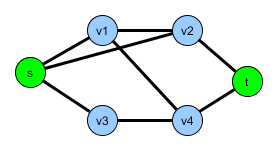
\includegraphics[width=5cm]{flow-problem-step-12-fig1.png}
	
	и сети, полученной из него по правилам в условии задачи:
	
	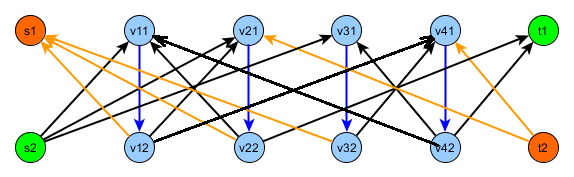
\includegraphics[width=13cm]{flow-problem-step-12-fig2.png}
	
	Для краткости буду называть вершины сети вида $v_{i1}$ чётными полувершинами (верхний ряд на рисунке), а вершины вида $v_{i2}$ -- чётными полувершинами.
	
	Во-первых, заметим, что только у стока (s2) допустим нулевой входной поток, а значит вершину t2 без входящих рёбер можно из рассмотрения выбросить. Поток из неё во все оранжевые рёбра всегда будет нулевым. Аналогично выбрасываем вершину s1 (у неё исходящиё поток тоже ноль) и идущие к ней оранжевые рёбра, т.к. поток через них всегда будет нулевым.
	
	Запустив на нашу сеть алгоритм Форда-Фалкерсона, мы найдём максимальный поток, который определяется (по теореме) минимальным S-T-разрезом. Попробуем угадать, какие рёбра в него войдут. Мы хотим получить разрез с минимальным потоком. Такие разрезы легче найти среди разрезов с минимальной пропускной способностью. Поскольку пропускная способность всех рёбер по правилам задачи одинакова и равна 1, мы ищем разрез с минимальным числом рёбер из S-половины в T-половину, причём рёбра, идущие из T в S (в обратном направлении) в разрезе не учитываются.
	
	Рассмотрим какую-нибудь пару полувершин, например $v_{11}$ и $v_{12}$. Если бы нечётная полувершина входила во множество T разреза, то мы бы учитывали входящие в неё рёбра из вершин s2, v22, v42. Если бы мы включили её в S-половину разреза вместе c s2, а v22 и v42 в T-половину, то все входящие в неё ребра не учитывались бы (все рёбра из зелёной s2 находятся внутри S-половины, а v22 и v42 были бы "обратными" $T \rightarrow S$-рёбрами). Учитывалось бы только единственное исходящее - вертикальное синее ребро $(v_{11} \rightarrow v_{12})$.
	
	Так же и в целом по построению сети ситуация такова: только синие рёбра (рёбра вида $v_{i1} \rightarrow v_{i2}$) идут сверху вниз, а все остальные снизу вверх. Поэтому минимальный S-T разрез будет иметь вид: S - это какое-то подмножество нечётных полувершин (верхний синий ряд) плюс s2, а T - какое-то подмножество чётных полувершин (нижний синий ряд) плюс t1. Соответственно рёбра в найденном минимальном разрезе будут из подмножества синих рёбер.
	
	Теперь заметим, что каждое синее ребро взаимно однозначно соответствует чётно-нечётной паре полувершин в $H$, т.е. их вершине-прототипу в $G$, и его удаление соответствует удалению этой вершины (т.е. удаление некоторого $(v_{i1} \rightarrow v_{i2})$ в $H$ однозначно соответствует удалению $v_i$ в $G$), а минимальный рёберный разрез по синим рёбрам в $H$ соответствует минимальному разделяющему множеству вершин в $G$.
	
	Найденный алгоритмом Форда-Фалкерсона максимальный поток -- это поток через минимальный рёберный разрез в $H'$ (какой бы он ни был, он будет среди синих рёбер) и соответвествует такому набору рёбер в $H$, что при его удалении путей между $s2$ и $t1$ не останется. Таким образом, максимальный поток в $H'$ даст нам размер минимального вершинно-разделяющего множества в $G$.
\end{proof}

\iiTODO



\section{Паросочетания}

\subsection{Задачи}

\begin{problem}
	Докажите, что любой кубический граф, имеющий не более двух мостов, можно покрыть путями длины 3, не пересекающимися по рёбрам.
\end{problem}
\begin{proof}
	В таком графе найдётся совершенное паросочетание. Удаляя его, мы получаем некоторый подграф. Каждая вершина в нём имеет степень 2. Значит, подграф состоит из циклов. Сориентируем рёбра каждого цикла графа в одном направлении:
	\begin{center}
		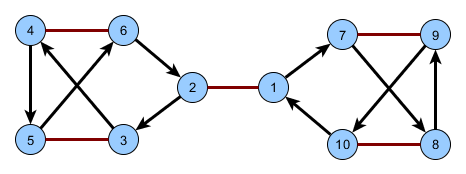
\includegraphics[width=10cm]{cubic-graph-cover-paths-3.png}
	\end{center}
	У каждой вершины будет одно входящее, одно исходящее и одно удалённое ``совершенное'' ребро. Пути длины 3 строим так: ребро ${u,v} \in M$, ребро исходящее из $v$, ребро исходящее из $u$.
\end{proof}

\begin{problem}
  Назовём граф критическим, если в нём нет совершенного паросочетания, но при удалении любой вершины оно появляется. Иначе говоря, для любой вершины в графе есть паросочетание,	покрывающее все вершины, кроме неё. Докажите, что $c_o(G \setminus S) - |S| \leqslant -1$ для любого непустого множества $S$ вершин критического графа.
\end{problem}
\begin{proof}
  Рассмотрим произвольное произвольное непустое множество $S$ в графе $G$
  и выделим произвольную (возможно, единственную, если $|S|=1$) вершину $x \in S$.
  Обозначим $G' = G \setminus x$ и $S' = S \setminus x$.
  Заметим, что $ |S| = |S'| + 1 $.
  Тогда:
  $ G \setminus S = G \setminus (S' \cup x) = (G \setminus x) \setminus S' = G' \setminus S' $.
  По условию задачи, в $G'$ всегда найдётся совершенное паросочетание, а значит:
  $ \mathrm{def}(G') = \max \limits_{\forall S'' \subset V'(G')} \big[ C_o(G' \setminus S'') - |S''| \big] = 0 $.
  Соединяя вместе эти формулы, получаем:
  $C_o(G \setminus S) - |S| = C_o(G' \setminus S') - (|S'| + 1) = \big[ C_o(G' \setminus S') - |S'| \big] - 1 \leqslant
   \max \limits_{\forall S'' \subset V'(G')} \big[ C_o(G' \setminus S'') - |S''| \big] - 1
   = \mathrm{def}(G') - 1 = 0 - 1 = -1 $
  Что и требовалось доказать. 
\end{proof}

\iiTODO


\subsection{Иллюстрации}

\begin{figure}[H]
	\centering
	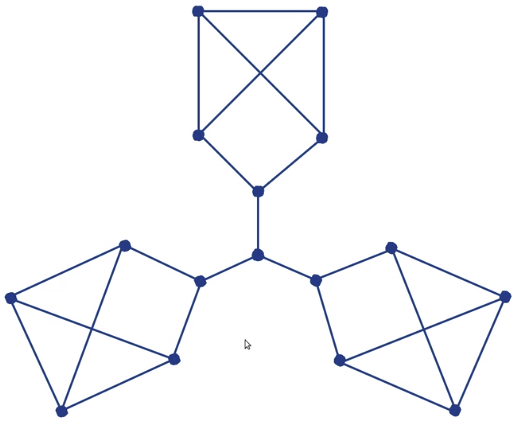
\includegraphics[width=7cm]{cubic-graph-example1.png}
	\caption{Кубический граф}
\end{figure}

\begin{figure}[H]
	\centering
	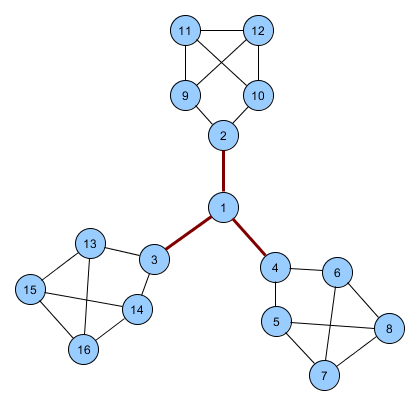
\includegraphics[width=9cm]{minimum-cubic-graph-with3-bridges.png}
	\caption{Мин. (16 вершин) кубический граф с 3 мостами (сов.п.с. $\nexists$)}
\end{figure}

\begin{figure}[H]
	\centering
	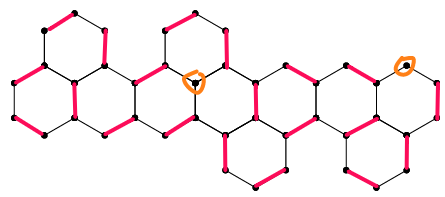
\includegraphics[width=10cm]{matching-deficit-2.png}
	\caption{Дефицит графа}
\end{figure}




\section{Раскраски}

\iiTODO




\section{Планарные графы I}

\begin{problem}
	Без использования теоремы о четырех красках доказать, что любой планарный связный граф, построенный на не более чем $n=11$ вершинах, является $4$-раскрашиваемым. \\
	Указание: вначале доказать, что в таком графе существует вершина, степень которой меньше или равна четырем.
\end{problem}
\begin{proof}
	
	Пусть $\delta = \min \limits_{v \in V(G)} \deg(v)$.
	Тогда $\delta \cdot V \leqslant \sum \limits_{v \in V(G)} {\deg(v)}
	      = 2E \leqslant 2(3V-6) = 6V-12$,
	поскольку для простых связных планарных графов верно $E \leqslant 3V-6$.
	Отсюда $ 12 / (6 - \delta) \leqslant V$.
	Но по условию $V \leqslant 11$, а значит $12 \leqslant 66 - 11 \delta$.
	Получаем, что $\delta \leqslant (54 / 11) \approx 4.9$,
	то есть целое число $\delta \leqslant 4$
	и найдется вершина $v$, у которой $\deg(v) \leqslant 4$.
	
	Теперь проведём рассуждение, полностью аналогичное приведённому на последней лекции, но вместо 5 цветов и соседей у нас будет 4.
	
	Проводим индукцию по количеству вершин. Для $V=4$ утверждение очевидно (а для меньшего числа тривиально/бессмысленно). Предположим, что для $(V-1)$ индукция уже доказана. Докажем теперь шаг индукции для $V$ ($V \leqslant 11$). Выделим вершину степени не больше 4 (мы показали, что она всегда найдётся), временно удалим, раскрасим остальной граф (это возможно по предположению шага) и вернём вершину на место. В худшем случае у вершины 4 соседа у которых 4 разных цвета (иначе раскрашиваем вершину 0 в оставшийся цвет). Например, 1-красный, 2-синий, 3-жёлтый, 4-зелёный, а самой вершине дадим индекс 0, как показано на рисунке.
	
	\begin{figure}[H]
		\centering
		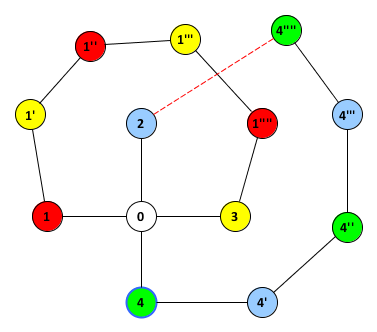
\includegraphics[width=8cm]{stepik-lesson12347-step8-problem.png}
	\end{figure}

	Сначала выбираем пару смежных вершин 1(красный)-3(жёлтый). Пытаемся перекрасить 1-ю в желтый, если же у неё есть жёлтый сосед 1', пытаемся перекрасить его в красный, при неудаче рассматриваем соседей соседа итд. Если удалось, меняем цвета в цепочке, 1-ю в жёлтый, 0-ю в красный и празднуем успех. В случае полной неудачи, худший случай - это когда цепочка дотянется до вершины 3. Тогда выбираем вторую пару 2(синий)-4(зелёный) и пытаемся перекрасить 4-ю в синий, а если найдётся синий сосед 4', пытаемся раскрасить его в зелёный, при неудаче тянем цепочку дальше. Рано или поздно сине-зелёная цепочка упрётся в красно-жёлтую, потому что та образует вместе с вершиной 0 замкнутый цикл, так что в этом случае удача нам гарантирована. Это доказывает шаг индукции и завершает задачу.
\end{proof}

\iiTODO


kuratovsky-task1-stage0.png

\section{Планарные графы II}

\begin{problem}
	Доказать с помощью теоремы Куратовского непланарность графа $G$, изображенного на рисунке:
	\\ 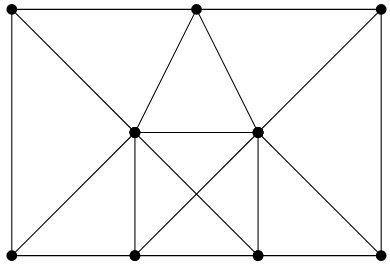
\includegraphics[width=3cm]{kuratovsky-task1-stage0.png}
\end{problem}
\begin{proof}
	Докажем, что подграф нашего графа, полученный \textit{удалением 4 рёбер}, является подразбиением графа $K_5$, что по критерию Куратовского гарантирует непланарность.
	\\ Пронумеруем вершины исходного графа:
	\\ 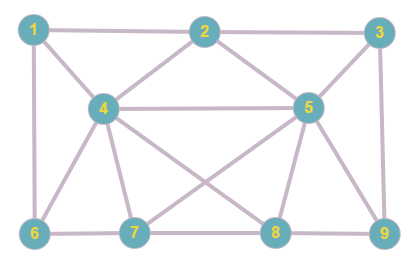
\includegraphics[width=5cm]{kuratovsky-task1-stage1.png}
	\\ В качестве подмножества для критерия возьмём граф, в котором удалены рёбра 4-1,4-6 слева и 5-3,5-9 справа:
	\\ 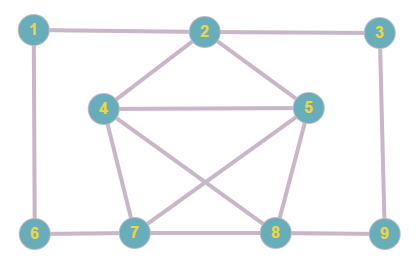
\includegraphics[width=5cm]{kuratovsky-task1-stage2.png}
	\\ Вершины 1,6,3,9 в результате имеют степень 2 и являются \textit{подразбиением} графа, к которому мы стремимся (для ясности немного переместим эти вершины):
	\\ 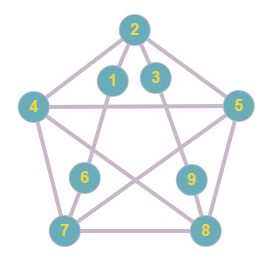
\includegraphics[width=5cm]{kuratovsky-task1-stage3.png}
	\\ Удалим подразбиения, заменив на прямые рёбра:
	\\ 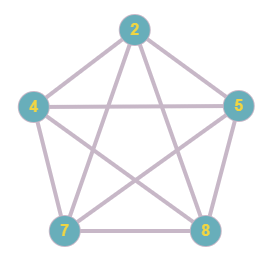
\includegraphics[width=5cm]{kuratovsky-task1-stage4.png}
	\\ Получившийся граф изоморфен графу $K_5$. Доказано.
\end{proof}


\begin{problem}
	Доказать с помощью теоремы Куратовского непланарность графа $G$, изображенного на рисунке:
	\\ 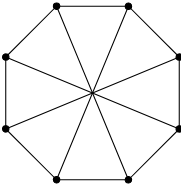
\includegraphics[width=3cm]{kuratovsky-task2-stage0-8angles.png}
\end{problem}
\begin{proof}
	Докажем, что подграф нашего графа, полученный \textit{удалением одного радиального ребра}, является подразбиением графа $K_{3,3}$, что по критерию Куратовского гарантирует непланарность.
	\\ Пронумеруем вершины исходного графа:
	\\ 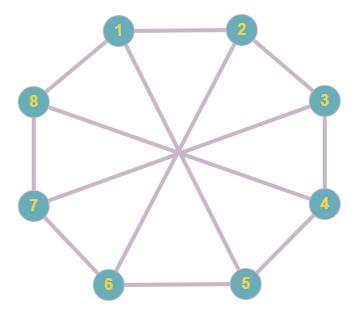
\includegraphics[width=5cm]{kuratovsky-task2-stage1.png}
	\\ В качестве подмножества для критерия возьмём граф, в котором удалено одно радиальное ребро, например ребро 4-8:
	\\ 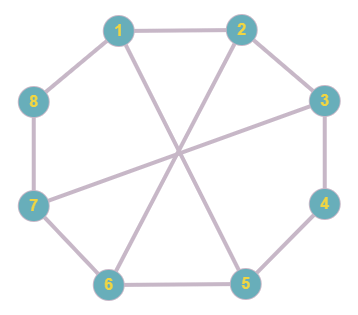
\includegraphics[width=5cm]{kuratovsky-task2-stage2.png}
	\\ Cмежные с удаленным ребром вершины 4,8 в подмножестве имеют степень 2 и являются \textit{подразбиением} графа, к которому мы стремимся. Удалим их, заменив на рёбра:
	\\ 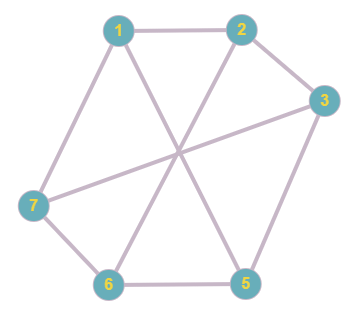
\includegraphics[width=5cm]{kuratovsky-task2-stage3.png}
	\\ Получившийся граф изоморфен графу $K_{3,3}$. Просто переставим вершины на рисунке для наглядности:
	\\ 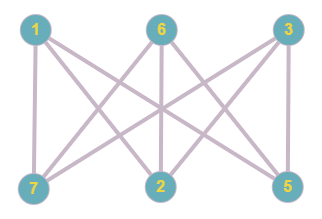
\includegraphics[width=5cm]{kuratovsky-task2-stage4.png}
	\\ Доказано.
\end{proof}


\begin{problem}
	Найти выпуклое вложение в плоскость графа $G$, показанного на рисунке:
	\\ 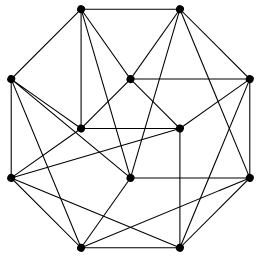
\includegraphics[width=3cm]{kuratovsky-task3-stage0.png}
\end{problem}
\begin{proof}
	Пронумеруем вершины исходного графа:
	\\ 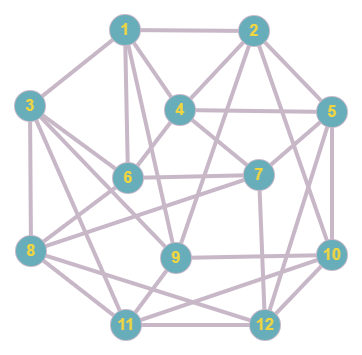
\includegraphics[width=7cm]{kuratovsky-task3-stage1.png}
	\\ И предъявим вложение:
	\\ 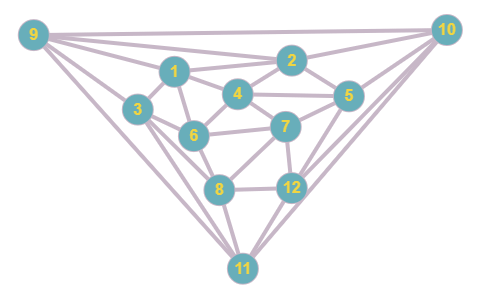
\includegraphics[width=9cm]{kuratovsky-task3-stage2.png}
\end{proof}


\iiTODO




\vspace{48pt} \noindent \hrulefill~ \raisebox{-8pt}[10pt][10pt]{\Huge\ding{102}}~ \hrulefill

\end{document}
